\documentclass{standalone}
\usepackage{pgfplots}
\usepgfplotslibrary{fillbetween}

\begin{document}
    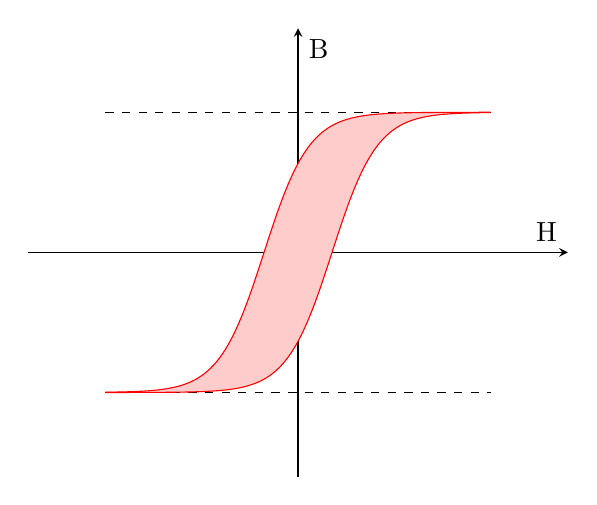
\begin{tikzpicture}
        \begin{axis}[very thick,
                     samples = 100,
                     xlabel = H,
                     ylabel = B,
                     xmin = -7,
                     xmax = 7,
                     ymin = -4,
                     ymax = 4,
                     axis x line = middle,
                     axis y line = middle,
                     ticks = none]
            \addplot[dashed] plot (\x, 2.5);
            \addplot[dashed] plot (\x,-2.5);
            \addplot[red, name path=A] plot (\x, {5/(1 + exp(-1.7*\x+1.5))-2.5});
            \addplot[red, name path=B] plot (\x, {5/(1 + exp(-1.7*\x-1.5))-2.5});
            \addplot[red!20] fill between[of=A and B];
        \end{axis}
    \end{tikzpicture}
\end{document}